\subsection{Audio Spatialisation}\label{subsec:audio-spatialisation}

Audio spatialisation is, plainly put, the practice of distributing sound in
space.
The spatialisation of \textit{primary sound sources}, e.g.\ sound
captured by microphones, stored as digital audio files, or synthesised in
real-time can be achieved simply by delivering those primary sources to
\textit{secondary sound sources}, i.e.\ loudspeakers or headphones.
%Loudspeakers being stationary entities by-and-large, the idea of moving a sound
%source is physically impractical, however, and that of locating a sound source
%between loudspeaker positions physically impossible.
Taking advantage of auditory cues, and the nature of the propagation of sound,
it is possible to suggest the presence of primary sources at arbitrary
locations, independent of the secondary source distribution.
The motivation behind audio spatialisation, then, is to create (or indeed
\textit{recreate}) sonic environments for creative and immersive purposes, such
as for virtual reality experiences, in cinematic settings, for music production
or art installations, to give but a handful of examples.

A number of techniques exist for what is termed \textit{sound field
synthesis}~\citep{ahrens_analytic_2012,nicol_sound_2017}, all of which
essentially take the form of applying some manner of \textit{driving function}
to an input audio signal to generate an appropriate driving signal to be
delivered to a secondary sound source in the listening
environment~\citep{ahrens_analytic_2012}.
For a loudspeaker at position $\mathbf{x} = \begin{bmatrix}
                                                x & y & z
\end{bmatrix}^T$, the time-domain driving signal $\hat{d}(\mathbf{x},t)$
can be expressed as a convolution of the input signal $\sigin(t)$ and the
driving function $d(\mathbf{x},t)$:
\begin{equation}
    \label{eq:driving-signal-time}
    \hat{d}(\mathbf{x},t) = \sigin(t) \ast d(\mathbf{x},t),
\end{equation}
where $t$ denotes time.


%the driving signal $\hat{D}(\mathbf{x}, \omega)$ can be
%expressed, in the frequency domain, as the product of the input signal,
%$\Sigin(\omega)$ and the driving function $D(\mathbf{x}, \omega)$:
%\begin{equation}
%    \label{eq:driving-signal-freq}
%    \hat{D}(\mathbf{x},\omega) = \Sigin(\omega) \cdot D(\mathbf{x},\omega),
%\end{equation}
%where $\omega$ denotes radian frequency, $\omega = 2\pi f$, and $f$, in turn,
%is time frequency.
%Moving to the time domain, the multiplication of the input signal and driving
%function changes to a convolution, and equation~\eqref{eq:driving-signal-freq}
%becomes:
%\begin{equation}
%    \label{eq:driving-signal-time}
%    \hat{d}(\mathbf{x},t) = \sigin(t) \ast d(\mathbf{x},t),
%\end{equation}
%where $t$ denotes time.

%An early sound field synthesis approach, referred to as an `acoustic
%curtain'~\citep{ziemer_wave_2020}, entailed placing microphones in one space,
%such as a concert auditorium, and, in another space, loudspeakers at locations
%corresponding to those of the microphones.
%In this case, there are as many input signals $\sigink(t)$ as there are
%microphones, and the driving function reduces to a `pass-through' of each
%signal to its corresponding loudspeaker, i.e.\
%$d_k(\mathbf{x}, t) = 1$.
%
%The acoustic curtain is a relatively rarely-deployed technique (though similar
%recreation of `real' sound fields is still conducted, albeit typically by way
%of ambisonic recording and reproduction) and sound field synthesis is most
%often concerned with the distribution and movement of artificial or arbitrary
%sound sources.

Commonly-employed approaches to sound field creation can be grouped into two
broad categories: amplitude- and time-based panning techniques, and physical
sound field recreation approaches.

\subsubsection{Periphony and Binaural Reproduction}\label{subsubsec:periphony}

The former, \textit{periphonic}, types encompass stereophony and surround-sound
systems, consisting of secondary sources in a horizontal planar arrangement
equidistant from the listening position.
These techniques exploit the interaural level difference (ILD) cue, i.e.\ the
difference in perceived amplitude relative to the listener's
ears~\citep{pulkki_virtual_1997,verheijen_sound_1998,ziemer_wave_2020}, to
encourage the listener to localise sound to a position on the circumference of
an arc or circle around the listening position.
%This is achieved by weighting the amplitudes of signals sent to the
%secondary sources, creating a ``phantom'' sound source that may appear to
%emanate from a position between loudspeakers.
For systems of this sort, the driving function is a constant scalar value, or,
for a moving phantom source, a time-varying function that returns a scalar
value.
Such periphonic approaches can extend to three dimensions in the case of
vector base amplitude panning (VBAP)~\citep{pulkki_virtual_1997}, which uses
trios of speakers to position phantom sources on the surface of a sphere
with the listening position at its origin.

Time-based panning effects, by contrast, make use of the interaural time
difference (ITD) cue to give the impression of a phantom source located toward
the loudspeaker producing the signal at the earliest
time~\citep{pulkki_virtual_1997,verheijen_sound_1998}.
Thus the driving function for a time-based panning system is a delay of the
form:
\begin{equation}
    d(\mathbf{x},t) = \delta(t - \tau),
    \label{eq:time-driving-function}
\end{equation}
where $\tau$ is the duration of the delay.

The effects of ILD and ITD cues transfer to headphone-based listening, in which
case, rather than periphonic, they form a sort of \textit{in-head}
localisation~\citep{ahrens_analytic_2012}.
For a significantly more naturalistic auditory outcome, ILD and ITD cues, when
combined with filters describing the dispersive and absorptive effects of the
head, torso and outer ears, constitute a Head-Related Transfer Function (HRTF),
the key component in what is termed \textit{binaural reproduction}.
Binaural recordings are taken either with a dummy head or ear-mounted
microphones, and thus the signal for each ear is coloured by the head used
during recording, or HRTF measurements can be taken and used to describe filters
to be applied to arbitrary signals at playback.
Binaural sound is suited to headphone-based listening but may be achieved with
loudspeakers if suitable cross-talk cancellation is
applied~\citep{kaiser_transaural_2011}.

%It is worth mentioning that these cues vary in their effectiveness with
%frequency and, excepting the case of headphone-based listening, intersect with
%cues related to listener's torso~\citep{verheijen_sound_1998} and the
%head-related transfer
%function~\citep{de_poli_physically_1998,geier_object-based_2010}.

Periphonic and binaural approaches are subject to the phenomenon of an ideal
listening position, or \textit{sweet-spot}~\citep{nicol_sound_2017}, that is a
listening position away from which the spatialisation effect is significantly
degraded.
Binaural reproduction, if not coupled with head motion tracking, is similarly
afflicted by an ideal position and
\textit{orientation}~\citep{verheijen_sound_1998};
further, for faithful reproduction, HRTFs should be
individualised~\citep{de_poli_physically_1998}.
As such, these techniques are not suited to collective and immersive auditory
experiences whereby multiple participants may move freely about their
environment.

%subjection to multiple listeners,
%nor to immersive auditory experiences permitting the participant to move freely
%about their environment.

%Additionally, phantom sources are inherently bound to the periphery on which
%they reside;
%there is no authentic way to model a phantom source at greater (or lesser)
%distance, though using reverberation and amplitude cues may offer a satisfactory
%perceptual impression.

\subsubsection{Physically-Inspired Techniques}\label{subsubsec:sound-field-synthesis}

\begin{figure}[ht]
    \centering
    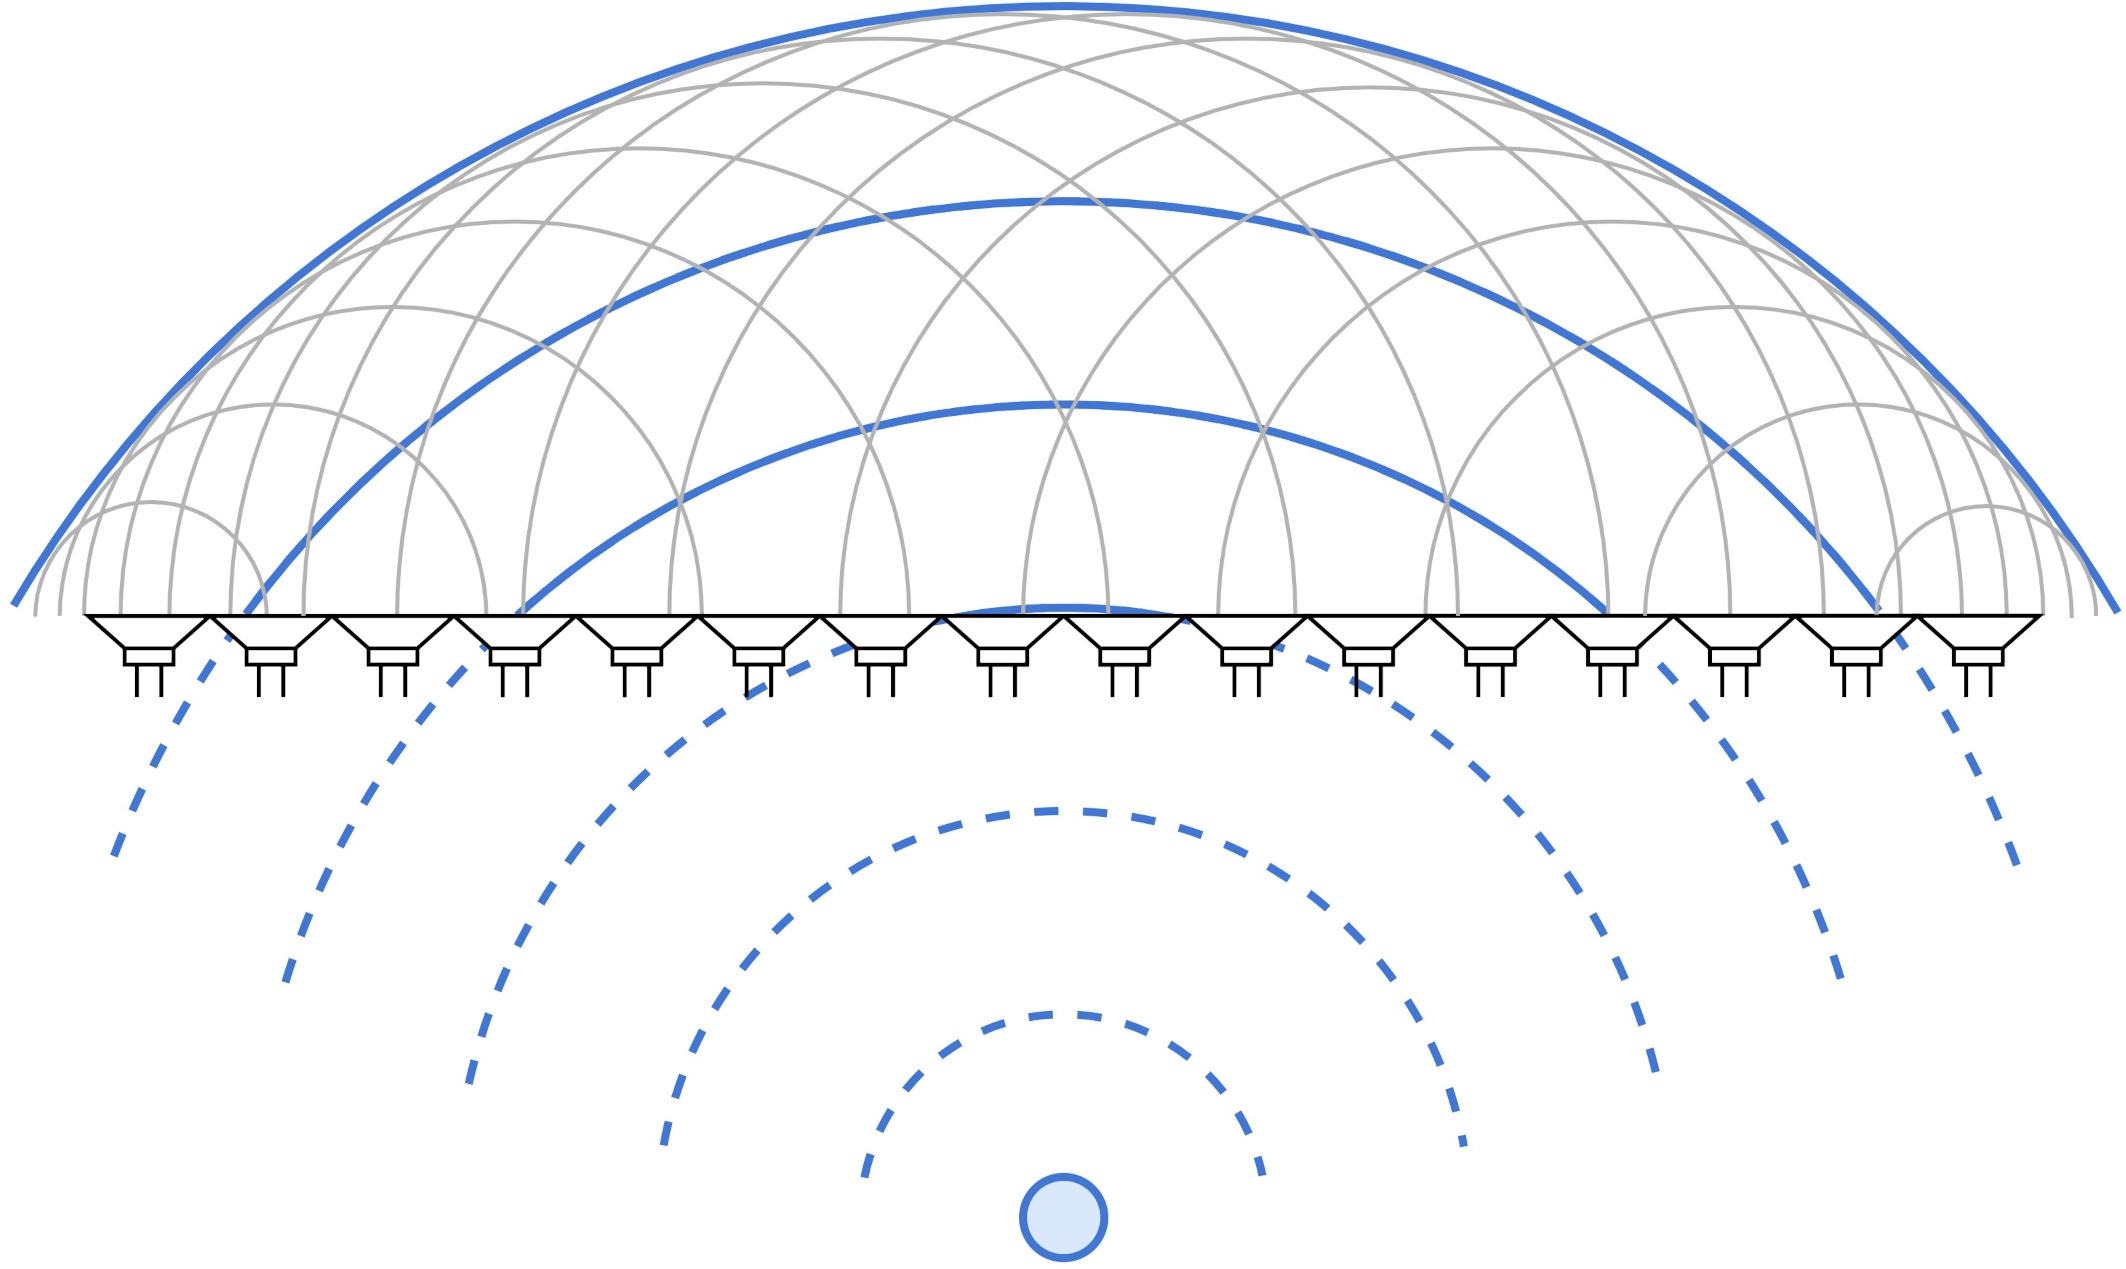
\includegraphics[width=.75\textwidth]{figures/wfs_1}
    \caption{\textit{Holophony}.
    Huygens' principle states that the propagation of a wavefront
    can be recreated by a collection of secondary point sources.
    The bottom of the figure represents a virtual sound field, and the top a
    real sound field, separated by a row of secondary point sources
        (loudspeakers).
        The small circle represents a virtual sound source and the dashed arcs
        are virtual wavefronts associated with that sound source;
        the small solid arcs are wavefronts produced by the array of secondary
        point sources;
        the large solid arcs represent the propagation of a reconstructed
        wavefront in the real sound field.}
    \label{fig:wfs_1}
\end{figure}

Physical approaches fall into two main types: wave field synthesis
(WFS)~\citep{berkhout_acoustic_1993} and
ambisonics (and higher-order ambisonics \textemdash{}
HOA)~\citep{frank_producing_2015}.
Rather than directly manipulating sound localisation cues, these types seek to
trigger those cues indirectly by synthesising a sound field as if it had been
created by `true' acoustic sources, as opposed to loudspeakers.
In the case of ambisonics, the sound field is decomposed into `spherical
harmonics', spatial functions described by linear sums of directional
components of increasing order~\citep{nicol_sound_2017}.
Spherical and plane waves can be reproduced, corresponding with virtual
point sources and sources at `infinite distance' respectively.

Ambisonics, like periphonic approaches, suffers from a sweet-spot effect which
worsens with attempts to reproduce sounds of higher frequency.
The ideal listening area can be broadened by implementing ambisonics at higher
order, increasing the density of the distribution of secondary sources.
Doing so obviously has ramifications for the physical complexity of an
ambisonics installation, and, since higher-order spherical modes must be
calculated, in terms of computational demands placed on the system.

\subsubsection{Wave Field Synthesis}

WFS is based upon Huygens' principle, originating in the field of optics, which
states that a propagating wavefront can be recreated by a distribution of
secondary point sources~\citep{mueller_acoustic_1971,berkhout_acoustic_1993,
    belloch_performance_2021} (see \figref{fig:wfs_1}).
It is variously termed a form of \textit{acoustic holography} or
\textit{holophony}~\citep{berkhout_holographic_1988,ahrens_analytic_2012}.
Effectively, by timing the reproduction of an input signal at an array of
secondary sources, a wavefront associated with a virtual sound source can be
synthesised.
To simulate distance cues, a filter can be applied to model losses to the
virtual medium of acoustic propagation.
The principle assumes a continuous array of secondary sources but of course in
practice it is necessary to use a discrete array of loudspeakers, which,
much as is the case with HOA, has consequences for spatial resolution;
to mitigate the issue of spatial aliasing, whereby sounds of higher frequency
cannot be recreated unambiguously~\citep{winter_geometric_2018}, secondary
sources should be placed very close together.
Consequently, to serve a large listening area, many speakers, and thus many
audio channels, are required.

Via appropriate timing of the delivery of a primary sound source to the
secondary source array, it is possible to synthesise virtual sound sources,
plane waves, and \textit{focused} sound sources, corresponding with concave,
flat, and convex synthesised wavefronts respectively; the latter, dependent
on the location of the listener, appear to emanate from within the real
sound field, rather than its virtual counterpart.

\begin{figure}[ht]
    \centering
    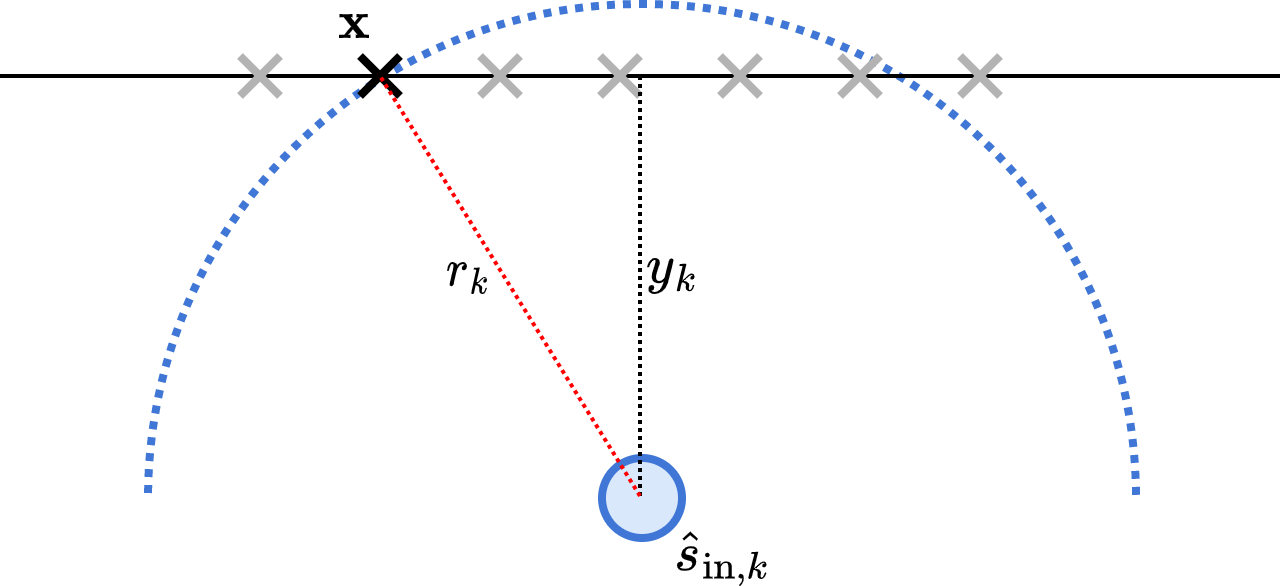
\includegraphics[width=.75\textwidth]{figures/wfs_2}
    \caption{
        The driving signal for the WFS secondary source at position $\bfx$,
        for virtual primary source $\sigink$, is dependent on the distance
        $r_k$ of the primary source from the secondary source.
        This corresponds with a propagation delay via the simulated medium of
        propagation, coupled with a filter describing losses to that medium.
    }
    \label{fig:wfs_2}
\end{figure}

Focusing on the former kind, however, for $m$ virtual sources, the time-domain
driving signal $\hat{d}$ for the secondary source at $\bfx$ may be expressed
as:
\begin{equation}
    \label{eq:driving-signal}
    \hat{d}(\bfx,t) = \sum_{k=0}^{m-1}\sigink \ast d_k(\bfx,t),
\end{equation}
where the driving function $d_k$ is~\citep{ahrens_analytic_2012}:
\begin{equation}
    \label{eq:driving-function}
    d_k(\bfx,t) = \frac{y_k}{r_k}f(t) \ast \delta\left(t - \frac{r_k}{c}\right).
\end{equation}
The \textit{WFS prefilter} $f(t)$ is a function that aims to simulate the
absorption of energy into the simulated medium of acoustic propagation.
The delta function $\delta$ has the effect of delaying the prefilter, and thus
$\sigink$, by the time of propagation for a medium with propagation speed $c$
(typically modelled as \qty[per-mode=symbol]{343}{\m\per\s} for sound in air).
The components of the driving function are depicted in \figref{fig:wfs_2}.

\subsubsection{State of the Art Spatial Audio Installations}
\label{subsubsec:spatial-sota}

A full 24-channel OTTOsonics system, including speakers and audio interface, is
costed at around \texteuro{2600}.
A more conventional, 64-channel WFS system, such as is installed in the
Multisensory Experience Lab at Aalborg University (AAU),
Copenhagen~\citep{grani_gestural_2016}, features two 32-channel MADI to analogue
converters costing roughly \texteuro{5000} apiece.
The world's largest WFS system, at TU Berlin, features over 800 output channels
driven by a distributed cluster of fifteen
computers~\citep{baalman_renewed_2007}\footnote{
    See also
    \url{https://tu.berlin/en/ak/research/projects/wellenfeldsynthese-fuer-einen-grossen-hoersaal}
    and WFS speaker module produced by Four Audio for installation at TU
    \url{https://four-audio.com/en/products/wfs/}.
}; the expense associated with this system is difficult to assess, as it is tied
to the concert hall space in which it resides.
Indeed, one thing besides expense that unites the systems at AAU and TU Berlin,
plus similar installations at IRCAM (Paris)\footnote{
    \url{https://ircam.fr/article/connaissez-vous-lespace-de-projection}
} and the Rensselaer Polytechnic Institute (NY, USA)\footnote{
    \url{https://empac.rpi.edu/about/building/venues}
} is their \textit{in-situ} nature;
these are site-specific systems with, at best, limited flexibility.
